\section{Análisis de la realimentación intermedia}
En esta sección se evalúa el comportamiento del sistema al prescindir de la realimentación del estado intermedio $x_2$. Físicamente, esto implica abrir el lazo correspondiente a la ganancia $k_2$.
\subsection{Análisis teórico a lazo cerrado}
A partir de la ecuación característica general del sistema realimentado obtenida previamente:
\begin{equation}
	|s\mathbb{I} - A + B\cdot k| = s^2 + s \cdot G_0 \cdot k_2 + G_0 \cdot k_1 = 0
\end{equation}

Al anular el camino de $k_2$ ($k_2 = 0$) y manteniendo $k_1 = 1$ para conservar la ganancia unitaria, la ecuación característica se reduce a:
\begin{equation}
	s^2 + G_0 = 0
\end{equation}

En consecuencia, la función de transferencia a lazo cerrado para este caso particular resulta:
\begin{equation}
	T(s) = \frac{G_0}{s^2 + G_0}
\end{equation}

Esta expresión corresponde a un sistema de segundo orden marginalmente estable, con un factor de amortiguamiento nulo ($\xi = 0$). Analíticamente, los polos del sistema se ubican sobre el eje imaginario puro en $s_{1,2} = \pm j\sqrt{G_0}$, lo que predice una respuesta oscilatoria sostenida.\\
De este modo, el sistema se interpretaria como:
\begin{figure}[H]
	\centering
	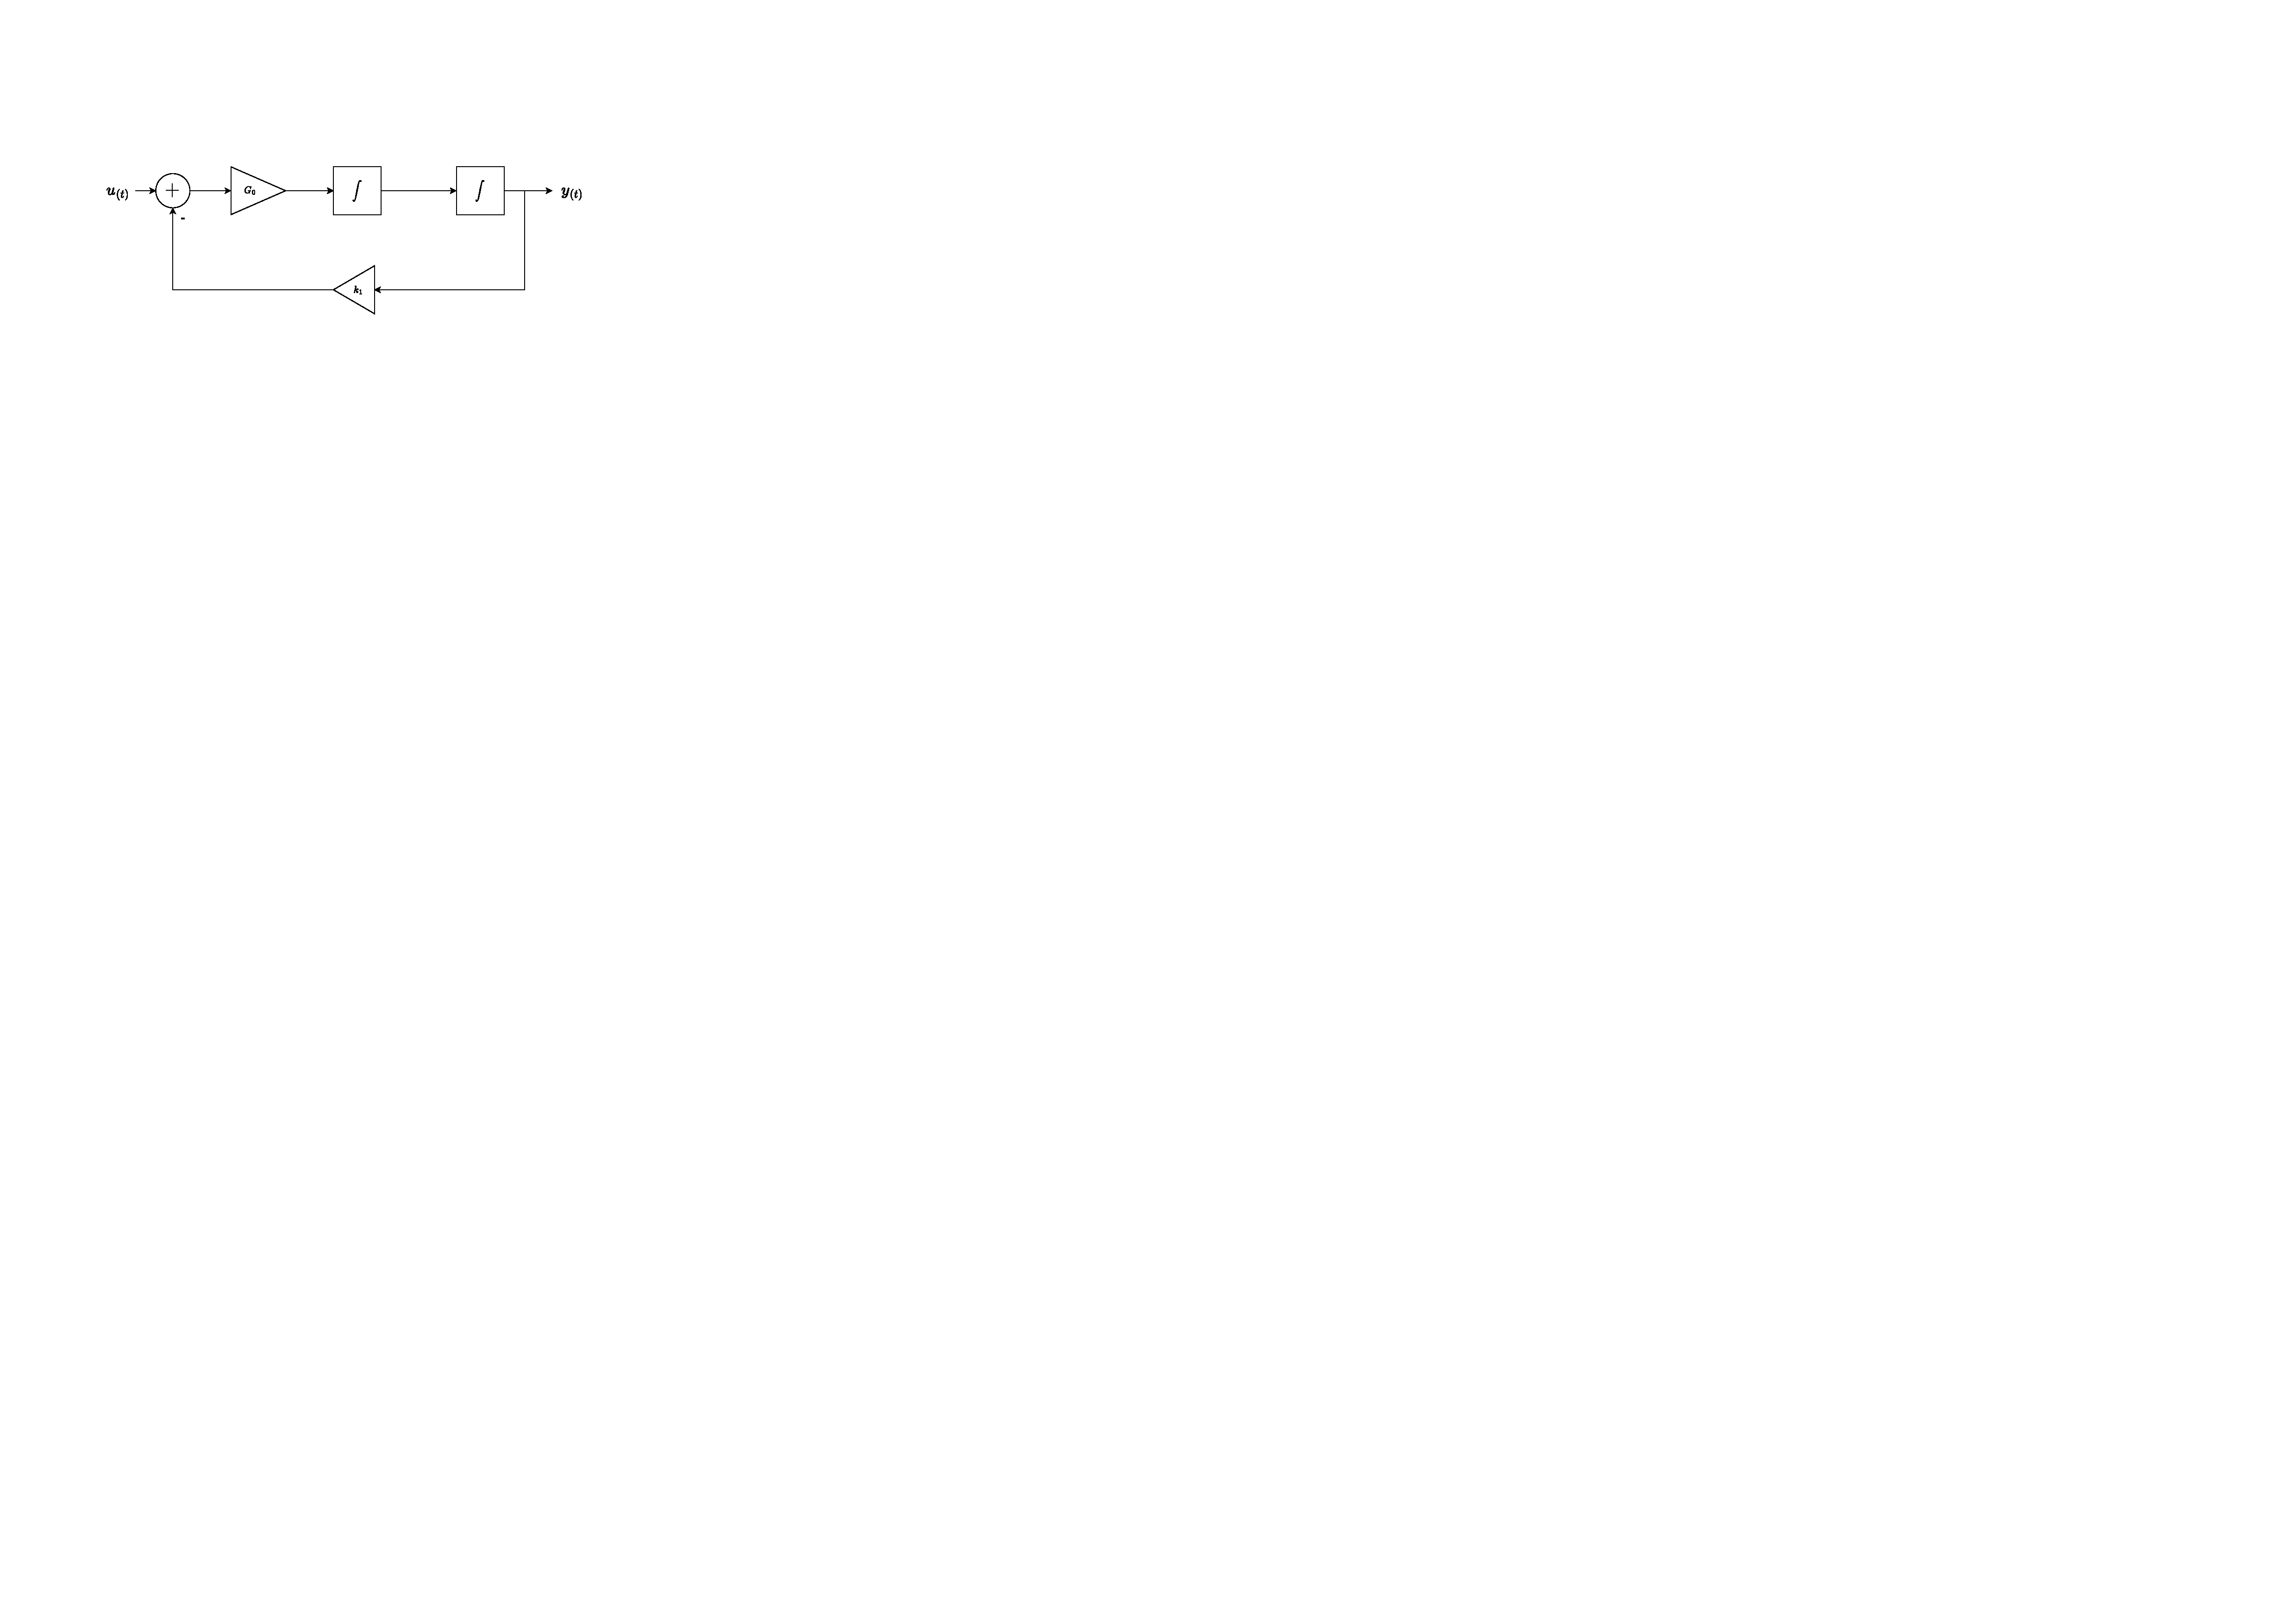
\includegraphics[width=0.9\textwidth]{Imagenes/5_Analisis_Retro-Int/lazo_cerrado-2.pdf} % Reemplazar con tu archivo
	\caption{Respuesta temporal con el camino $k_2$ abierto: Simulación vs. Medición.}
	\label{fig:step_k2_open}
\end{figure}
\newpage
\subsection{Respuesta temporal: Simulación vs. Medición}
Al simular el modelo analítico (Matlab) sin $k_2$, el sistema oscila de forma sostenida entre 0V y 2.00V, congruente con el modelo matemático ideal. 

Sin embargo, al medir la respuesta en el circuito físico (Figura \ref{fig:step_k2_open}), se registra una oscilación amortiguada que decae progresivamente durante aproximadamente 25 segundos hasta estabilizarse cerca de 1.00V.

\begin{figure}[H]
	\centering
	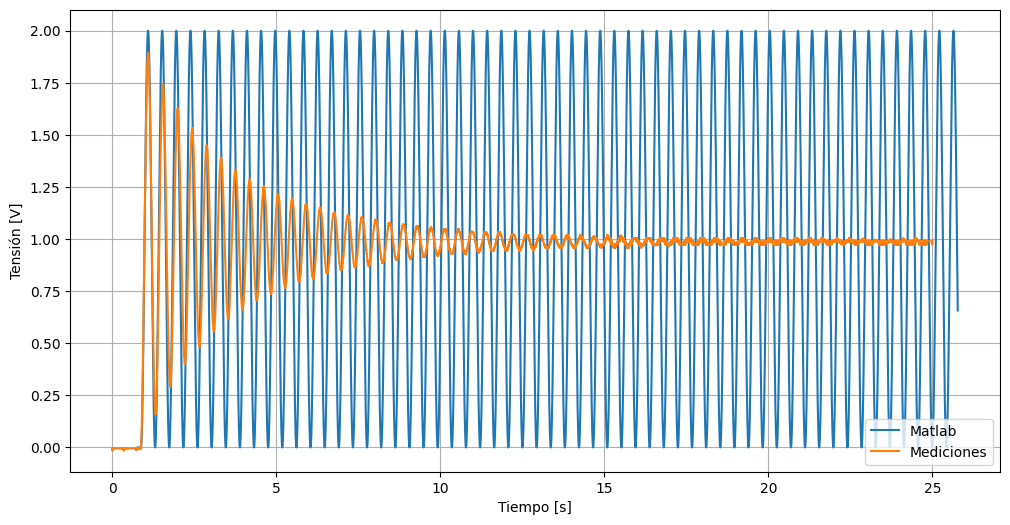
\includegraphics[width=0.9\textwidth]{Imagenes/5_Analisis_Retro-Int/2_Lazo-Abierto.png} % Reemplazar con tu archivo
	\caption{Respuesta temporal con el camino $k_2$ abierto: Simulación vs. Medición.}
	\label{fig:step_k2_open}
\end{figure}

Esta diferencia fundamental se justifica por las características no ideales de los componentes físicos. Los amplificadores operacionales reales presentan anchos de banda finitos, resistencias de salida no nulas y corrientes de polarización que, junto con las tolerancias y pérdidas en los capacitores, introducen un amortiguamiento parásito en el sistema. Este efecto disipativo intrínseco provoca que los polos reales del circuito se desplacen levemente hacia el semiplano izquierdo, garantizando la estabilidad asintótica observada en la práctica.
\newpage
\subsection{Análisis en el Plano de Fase}
Para complementar el análisis, se trazó el plano de fase (Derivada de la Salida vs. Salida) para este escenario. 

Como se observa en la Figura \ref{fig:fase_k2_open}, la simulación teórica muestra un ciclo límite casi perfecto (círculo exterior continuo), lo cual es el comportamiento característico de una oscilación sostenida sin amortiguamiento. La medición física, por el contrario, traza una espiral densa que converge lentamente hacia el centro, evidenciando nuevamente la paulatina disipación de energía del circuito real a lo largo del tiempo.

\begin{figure}[H]
	\centering
	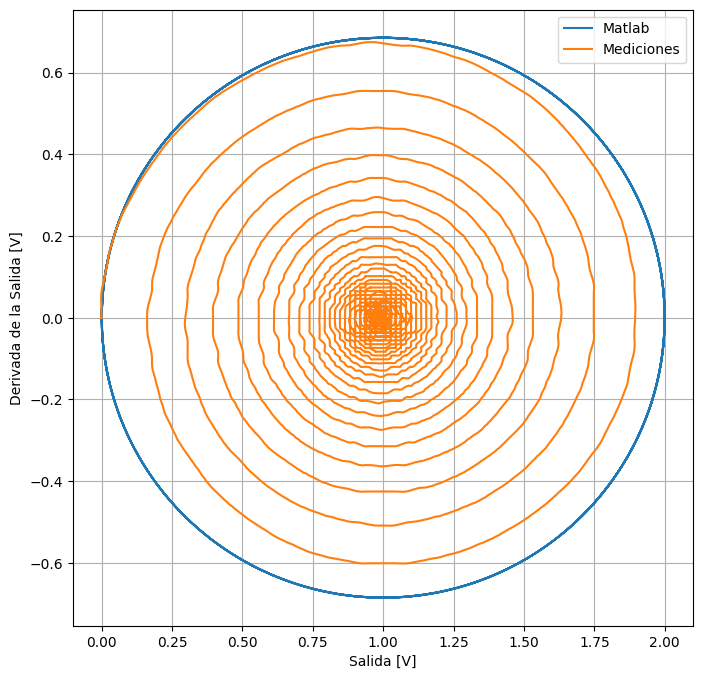
\includegraphics[width=0.7\textwidth]{Imagenes/5_Analisis_Retro-Int/4_Fase-Abierto.png} % Reemplazar con tu archivo
	\caption{Plano de fase del sistema con el camino $k_2$ abierto.}
	\label{fig:fase_k2_open}
\end{figure}